\documentclass[12pt]{article}
\usepackage[paper=letterpaper,margin=1.5cm]{geometry}
\usepackage{amsmath}
\usepackage{amssymb}
\usepackage{amsfonts}
\usepackage{mathtools}
%\usepackage[utf8]{inputenc}
%\usepackage{newtxtext, newtxmath}
\usepackage{lmodern}     % set math font to Latin modern math
\usepackage[T1]{fontenc}
\renewcommand\rmdefault{ptm}
%\usepackage{enumitem}
\usepackage[shortlabels]{enumitem}
\usepackage{titling}
\usepackage{graphicx}
\usepackage[colorlinks=true]{hyperref}
\usepackage{setspace}
\usepackage{subfigure} 
\usepackage{braket}
\usepackage{color}
\usepackage{tabularx}
\usepackage[table]{xcolor}
\usepackage{listings}
\usepackage{mathrsfs}
\usepackage{stackengine}
\usepackage{physics}
\usepackage{afterpage}
\usepackage{pdfpages}
\usepackage[export]{adjustbox}
\usepackage{biblatex}

\setstackEOL{\\}

\definecolor{dkgreen}{rgb}{0,0.6,0}
\definecolor{gray}{rgb}{0.5,0.5,0.5}
\definecolor{mauve}{rgb}{0.58,0,0.82}


\lstset{frame=tb,
  language=Python,
  aboveskip=3mm,
  belowskip=3mm,
  showstringspaces=false,
  columns=flexible,
  basicstyle={\small\ttfamily},
  numbers=none,
  numberstyle=\tiny\color{gray},
  keywordstyle=\color{blue},
  commentstyle=\color{dkgreen},
  stringstyle=\color{mauve},
  breaklines=true,
  breakatwhitespace=true,
  tabsize=3
}
\setlength{\droptitle}{-6em}

\makeatletter
% we use \prefix@<level> only if it is defined
\renewcommand{\@seccntformat}[1]{%
  \ifcsname prefix@#1\endcsname
    \csname prefix@#1\endcsname
  \else
    \csname the#1\endcsname\quad
  \fi}
% define \prefix@section
\newcommand\prefix@section{}
\newcommand{\prefix@subsection}{}
\newcommand{\prefix@subsubsection}{}
\renewcommand{\thesubsection}{\arabic{subsection}}
\makeatother
\DeclareMathOperator*{\argmin}{argmin}
\newcommand{\partbreak}{\begin{center}\rule{17.5cm}{2pt}\end{center}}
\newcommand{\alignbreak}{\begin{center}\rule{15cm}{1pt}\end{center}}
\newcommand{\tightalignbreak}{\vspace{-5mm}\alignbreak\vspace{-5mm}}
\newcommand{\hop}{\vspace{1mm}}
\newcommand{\jump}{\vspace{5mm}}
\newcommand{\R}{\mathbb{R}}
\newcommand{\C}{\mathbb{C}}
\newcommand{\N}{\mathbb{N}}
\newcommand{\G}{\mathbb{G}}
\renewcommand{\S}{\mathbb{S}}
\newcommand{\bt}{\textbf}
\newcommand{\xdot}{\dot{x}}
\renewcommand{\star}{^{*}}
\newcommand{\ydot}{\dot{y}}
\newcommand{\lm}{\mathrm{\lambda}}
\renewcommand{\th}{\theta}
\newcommand{\id}{\mathbb{I}}
\newcommand{\si}{\Sigma}
\newcommand{\Si}{\si}
\newcommand{\inv}{^{-1}}
\newcommand{\T}{^\intercal}
\renewcommand{\tr}{\text{tr}}
\newcommand{\ep}{\varepsilon}
\newcommand{\ph}{\varphi}
%\renewcomand{\norm}[1]{\left\lVert#1\right\rVert}
\definecolor{cit}{rgb}{0.05,0.2,0.45}
\addtolength{\jot}{1em}
\newcommand{\solution}[1]{

\noindent{\color{cit}\textbf{Solution:} #1}}

\newcounter{tmpctr}
\newcommand\fancyRoman[1]{%
  \setcounter{tmpctr}{#1}%
  \setbox0=\hbox{\kern0.3pt\textsf{\Roman{tmpctr}}}%
  \setstackgap{S}{-.9pt}%
  \Shortstack{\rule{\dimexpr\wd0+.1ex}{.9pt}\\\copy0\\
              \rule{\dimexpr\wd0+.1ex}{.9pt}}%
}

\newcommand{\Id}{\fancyRoman{2}}

% Enter the specific assignment number and topic of that assignment below, and replace "Your Name" with your actual name.
\title{STAT 31020: Homework 2}
\author{Caleb Derrickson}
\date{Wednesday, January 17, 2022}

\begin{document}
\onehalfspacing
\maketitle
\allowdisplaybreaks


\tableofcontents

\newpage
\section{Problem 1}
We call an analytical function in the domain $D \subset \R$, $D$ and open set, an infinitely differentiable function for which the Taylor series at x converges at every point $y \in N(x) \subset D$ to the value of the function at $y$, $f(y)$.

\subsection{Problem 1, part a}
Prove that for an analytical function on $\R$ a necessary and sufficient condition for $x$ to be an isolated local minimum is for $k(x)$ in problem 1, homework 1, to be even, positive, and for $f$ to satisfy $f^{(k(x))}(x) > 0$.
\partbreak
\begin{solution}

    I will assume necessary and sufficient conditions are impinged on showing $x$ is an isolated local minimum if and only if $k(x)$ is positive, even, and $f^{(k(x))}(x) > 0$. For simplicity, I will take $x^*$ to be the isolated local minimum, $k(x)$ to be expressed simply as $k$, and $N(x)$ to be expressed as $N$. \par

    \jump 
    For the forward direction, we will assume that $x^*$ is an isolated local minimum within a Neighborhood $N$ of $x^*$. Thus $f(x^*) < f(x)$ for all $x \in N$\footnote{Within the neighborhood, isolated local minimum implies strict local minimum.}. By Taylor's Theorem, and since $f$ is given as infinitely differentiable, we can express $f(y)$ for any $y \in N$ as
    \[f(y) = f(x^*) + \sum_{j = 1}^\infty \frac{1}{j!}f^{(j)}(x^*)(y - x^*)^{(j)}\]
    Note that $k$ is the first nonzero derivative of $f(x^*)$. Within this neighborhood, we can approximate the value of $f(y)$ by the investigation of two terms, 
    \[f(y) \approx f(x^*) + \frac{1}{k!}f^{(k)}(x^*)(y - x^*)^{(k)}.\]
    Since $x^*$ is a strict local minimum within the neighborhood, $f(y) - f(x^*) > 0$. This means
    \[f^{(k)}(x^*)(y - x^*)^{(k)} > 0,\]
     where the factor of $1 / k!$ was discarded. This statement implies the signs of both terms $f^{(k)}(x^*)$ and $(y - x^*)^{(k)}$ are equal. Thus, we can break this down into two cases:

     \begin{itemize}
         \item \underline{Case 1:} $f^{(k)}(x^*) < 0$ and $(y - x^*)^{(k)} < 0$.
         
         \jump
         Considering the second term, we see that $(y - x^*)^{(k)} < 0$. This implies that $k$ is odd, since if $k$ were even, then $k = 2m$ for $m \in \N$, so $(y - x^*)^{(k)} = (y - x^*)^{(2m)}$, which is strictly positive. Note that $y \neq x^*$ by assumption. Thus $k$ is odd. Note that we are investigating around an open ball of $x^*$, so the expression $y - x^*$ could be either positive or negative. If we consider $y > x^*$, then $y - x^* > 0$, so $(y - x^*)^{(k)} > 0$. This is a contradiction, since $(y - x^*)^{(k)} < 0$. Thus $f^{(k)}(x^*) < 0$ and $(y - x^*)^{(k)} < 0$ cannot be true.

         \item \underline{Case 2:} $f^{(k)}(x^*) > 0$ and $(y - x^*)^{(k)} > 0$.

         \jump
         We will again only consider the second term. Here, since we are investigating around an open ball of $x^*$ $y - x^*$ could be either positive or negative. In the previous case, we saw that the condition $(y - x^*)^{(k)} < 0$ restricted us to only considering $k$ odd. Since $(y - x^*)^{(k)} > 0$, this restricts to $k$ being even.\footnote{Or, we only restrict values for which $y > x^*$. This gives the contradiction from Case 1.} Therefore, by exhaustion of cases, and consideration of the two terms, we see that $f^{(k)}(x^*) > 0$ and $k$ even. We also have that $k$ is positive, by the Taylor series expansion. Thus the forward direction is shown.
     \end{itemize}

     \jump
     For the backward direction, we have that $k$ is even, positive, and that $f^{(k)}(x^*) > 0$. We wish to show that $x^*$ is an isolated local minimum for $N$. We will again consider the Taylor series approximation for any $y$ within a local neighborhood $N$ of $x^*$ as 
     \[f(y) \approx f(x^*) + \frac{1}{k!}f^{(k)}(x^*)(y - x^*)^{(k)}.\]
     We are given that $f^{(k)}(x^*) > 0$. Furthermore, note that since $k$ is even (and positive), we note that $(y - x^*)^{(k)} > 0$ for $y \neq x^*$. We then see that  
     \[f(y) - f(x^*) = \frac{1}{k!}f^{(k)}(x^*)(y - x^*)^{(k)} > 0.\]
     Therefore, $f(y) > f(x^*)$ for $y \in N\setminus\{x^*\}$. Therefore, $x^*$ is an isolated local minimum. 
\end{solution}
\newpage
\subsection{Problem 1, part b}
What can you then say about the function that you used as an example at problem 1 homework 1, part 4?
\partbreak
\begin{solution}
    
\end{solution}

\newpage
\section{Problem 2}
Prove Zoutendijk's Theorem (Theorem 3.2 stated in the book) for the case where the step length $\alpha_k$ is computed by backtracking, but starting at fixed $\Tilde{\alpha} > 0$. For this to work, assume in the following there exists some $c_3 > 0$ such that the search direction $p_k$ satisfies $\norm{p_k} \geq c_3 \norm{\nabla f(x_k)}$. Explain how the conclusion may fail if you do not impose this condition.
\partbreak
\begin{solution}

    I will provide the Theorem below.
    \tightalignbreak
    \begin{quote}
        Consider any iteration of the form $x_{k+1} = x_k + \alpha_k p_k$, where $p_k$ is a descent direction and $\alpha_k$ satisfies the Wolfe conditions. Suppose that $f$ is bounded below in $\R^n$ and that $f$ is continuously differentiable in an open set $N$ containing the level set $L \stackrel{\text{def}}{=} \{ x : f(x) \leq f(x_0)\}$, where $x_0$ is the starting point of the iteration. Assume also that the gradient $\nabla f$ is Lipschitz continuous on $N$, that is, there exists a constant $L > 0$ such that 
        \[\norm{\nabla f(x) - \nabla f(\Tilde{x})} \leq L\norm{x - \Tilde{x}}, \quad \text{for all } x, \Tilde{x} \in N.\]
        Then
        \[\sum_{k \geq 0} \cos^2\theta_k \norm{\nabla f_k}^2 < \infty.\]
    \end{quote}
    \vspace{-6mm}\alignbreak

    
\end{solution}

\newpage
\section{Problem 3}
Consider an optimization problem $\min_{x \in \R^n} f(x)$ where $f$ is twice continuously differentiable. Assume that $x^*$ is a local solution that satisfies the first order necessary condition $\nabla f(x^*) = 0$ and the second-order sufficient condition $\nabla_{xx}^2f(x^*) \succ 0$.
\subsection{Problem 3, part a}
Prove that, there exists parameters $c_1, c_2 > 0$ such that for all $x$ sufficiently close to the local solution we have that $c_1 \norm{x - x^*} \leq \norm{\nabla f(x)} \leq c_2\norm{x - x^*}$ 
\partbreak
\begin{solution}

    We first note that the Hessian $\grad ^2 f(x\star)$, so in a neighborhood $D$ around the critical point $x\star$, the function $f|_{D}$ is convex. Therefore, the gradient $\grad f(x)$ is Lipschitz in $D$. The right inequality is simple. Since $\grad f$ is lipschitz continuous, for some $L > 0$, we can say for any $x, y$ in a neighborhood of $x\star$
    \[\norm{\grad f(x) - \grad f(y)} \leq L \norm{x - y}.\]
    Setting $y = x\star$, and noting that $\grad f(x\star) = 0$, we get 
    \[\norm{\grad f(x)} \leq L \norm{x - x\star}.\]
    Therefore, setting $c_2 = L$ satisfies the right inequality for any $x$ in a neighborhood of our local minima. For the left hand side, we can first note by the Fundamental Theorem of Calculus, 
    \[\int_x^{x\star} \grad f(x') \cdot \textbf{dx'} \leq \left | \int_x^{x\star} \grad f(x') \cdot \textbf{dx'} \right | \leq \int_x^{x\star} \norm{\grad f(x')} \norm{\textbf{dx'}}.\]
    Since $\textbf{dx'}$ is a unit vector in the direction of integration, the integral is just the value $\norm{\grad f(x)}$. Relating this to the distance from $x$ to $x\star$, we can take a Taylor expansion of $f$.
    \[f(x) = f(x\star) + \grad f(x\star)(x - x\star) + \frac{1}{2}(x - x\star)^\intercal \grad^2 f(x\star)(x - x\star).\]
    $x\star$ is a local minimizer, so after simplification and rearranging,
    \[f(x) - f(x\star) = \frac{1}{2}(x - x\star)^\intercal \grad^2 f(x\star)(x - x\star).\]
    Therefore, 
    \[|f(x) - f(x\star)| = \frac{1}{2}|(x - x\star)^\intercal \grad^2 f(x\star)(x - x\star)| \leq \norm{x - x\star}\norm{\grad^2 f(x)}.\]
    Combining this with what we found before, we get
    \[\frac{\norm{\grad^2f(x\star)}}{2}\norm{x - x\star} \leq \norm{\grad f(x)}.\]
    Since $\grad^2f(x\star)$ is positive definite, its norm is positive. So setting $c_1 = \frac{1}{2}\norm{\grad^2f(x\star)}$ will satisify the inequalities. 
\end{solution}
\newpage
\subsection{Problem 3, part b}
Use this result to prove that under the sufficient conditions, not only is $x^*$ a strict local minima, but also an isolated local minimum. 
\partbreak
\begin{solution}

    Suppose there is a neighborhood $N$ around $x^*$ such that the second order Taylor Expansion at $y \in N$ is a fine approximation. That is,
    \[f(y) = f(x^*) + \grad f(x^*)(y - x^*) + \frac{1}{2}(y - x\star)\grad ^2f(x\star)(y - x\star).\]
    Since $\grad f(x\star) = 0$, the second term is cancelled. After rearranging, 
    \[f(y) - f(x) = \frac{1}{2}(y - x\star)\grad ^2f(x\star)(y - x\star)\]
    Since $\grad^2 f(x\star) \succ 0$, we have that for any $z \in N, \ z^T \grad^2f(x\star)z > 0$. Thus the right side is greater than zero, meaning $f(y) - f(x\star) > 0$, which means $f(y) > f(x\star)$ for any $y \in N$. Thus, $x\star$ is an isolated local minima.
\end{solution}

\newpage
\subsection{Problem 3, part c}
Assume now that you have an algorithm that produces a sequence $x_k \rightarrow x\star$ such that the gradient sequence $\norm{\grad f(x_k)}$ converges R-linearly to zero. What can you say about the convergence of the error sequence $\norm{x_k - x\star}$? 
\partbreak
\begin{solution}

    We have that $\norm{\grad f(x_k)} \rightarrow 0$ R-linearly. By definition, there exists a sequence $\{v_k\}$ satisfying $\norm{\grad f(x_k)} \leq v_k$ for all $k$, where $v_k$ converges Q-linearly to zero. From part a, we have that there exists $c_1 > 0$ such that $c_1 \norm{x_k - x\star} \leq \norm{\grad f(x)}$. By transitivity, $\norm{x_k - x\star} \leq \frac{1}{c_1}v_k$ for all $k$. \footnote{If $x_k$ is does not start in a sufficient neighborhood, extract a subsequence that is then in the neighborhood.} Defining a new sequence $w_k = \frac{1}{c_1}v_k$, we can see that $w_k$ converges Q-linearly to zero as well, since 
    \[\frac{w_{k+1}}{w_k} = \frac{(1/c_1)v_{k+1}}{(1/c_1)v_k)} = \frac{v_{k+1}}{v_k} < r < 1.\]
    Therefore, we can say the sequence $x_k$ converges R-linearly to $x^*$, so $\norm{x_k - x\star}\rightarrow 0$.
\end{solution}

\newpage
\subsection{Problem 3, part d}
Assume now that you have an algorithm that produces a sequence $x_k \rightarrow x\star$ such that the gradient sequence $\norm{\grad f(x_k)}$ converges R-superlinearly to zero. What can you say about the convergence of the error sequence $\norm{x_k - x\star}$?
\partbreak
\begin{solution}

    In the same spirit as the last part, we have that $c_1\norm{x_k - x\star} \leq \norm{\grad f(x_k)} \leq v_k$ for some sequence $v_k$ which converges to zero Q-superlinearly. Then $x_k$ converges R-superlinearly as well, since it is bounded by a Q-superlinear sequence.  
\end{solution}

\newpage
\subsection{Problem 3, part e}
Assume now that there is an optimization algorithm that is convergent to $x\star$. Propose a computable test to decide whether the sequence is superlinearly or quadratically convergent.
\partbreak
\begin{solution}

    Since we have no knowledge of a limit, I would imagine that we could analyse the forward error of the sequence $x_k$. That is, we would expect the sequence $\norm{\grad f(x_k) - \grad f(x\star)}$ to converge to zero. Since $x\star$ would be a local minima, th first order necessary conditions would hold. So $\grad f(x\star) = 0$, meaning the forward error simplifies to $\norm{\grad f(x_k)}$. We see that this bounds the sequence $\norm{x_k - x\star}$, so $\norm{x_k - x\star}$ will converge when $\norm{\grad f(x_k)}$ converges to zero. Therefore, the rate of convergence of $x_k$ to $x\star$ depends entirely on the convergence of $\norm{\grad f(x_k)}$. So if $\norm{\grad f(x_k)}$ is R-quadratically convergent, then so is $x_k$, and the same for R-superlinear convergence.
\end{solution}


\newpage
\section{Problem 4}
\subsection{Problem 4, part 1}
Implement the steepest descent algorithm as discussed in the class using the backtracking (Armijo) algorithm 3.1 from the textbook. We will apply it to the quadratic function $f(x) = x_1^2 + cx_2^2, c > 0$ in various circumstances that I will describe below. The solution to its minimization is $(0, 0)$. 
\partbreak
\begin{solution}

    I have implemented this, where all you need to do is call calebderrickson\_hw2p4(x0, c) when you are in the folder. It will output two plots, one showing the normed gradient sequence as described in problem 3, and the ratio of normed gradient sequences. The script will also print out the number of iterations, as well as the estimate on the minima.
\end{solution}

\newpage
\subsection{Problem 4, part 2}
There is a theorem (3.3) that tells you what a bound on the rate of convergence could be, though for a different line search type, but we will use it as a yardstick. What is that bound as a function of $c$?
\partbreak
\begin{solution}

    The bound is given as 
    \[\left ( \frac{\lm_n - \lm_1}{\lm_n + \lm_1}\right ),\]
    where $0 < \lm_1 \leq \lm_2 \leq ... \leq \lm_n$ are the eigenvalues of $Q$, a symmetric positive definite matrix, where our $f$ is of the form $f(x) = \frac{1}{2}x^\intercal Qx - b^\intercal x$. Though not exactly similar, for all intensive purposes, we can assume $Q$ is the Hessian of our function. Therefore, we take $Q$ as
    \[Q = \grad ^2 f = \mqty[2&0\\0&2c]\]
    Therefore, the eigenvalues of $Q$ are 2 and $2c$. Although not explicitly told, for all parts of this problem, we take $c \geq 1$, so the ordering of eigenvalues are $\lm_1 = 2, \ \lm_2 = 2c$. This then gives our bound as 
    \[\left ( \frac{c - 1}{c + 1}\right ).\]

\end{solution}

\newpage
\subsection{Problem 4, part 3}
Propose a method to track the convergence without making use of the information about where the minimum is. Can you think of ways to use this information to check the rate of convergence (and what rate can you hope to obtain)? Discuss your rationale.
\partbreak
\begin{solution}

    From Problem 3, we can take convergence to a minimum when our sequence of points $x_k$ has the property that $\norm{\grad f(x_k)} \rightarrow 0$ as $k \rightarrow \infty$. Checking the rate of convergence, we can take it as the ratio of sequential values of the normed-gradient. We will encounter floating point / cancellation errors as we get closer to the minima, however. This will be ignored for the moment, and be assuaged if necessary. 
\end{solution}

\newpage
\subsection{Problem 4, part 4}
Propose a stopping criterion based on 2, that is, when would it seem it does not make sense to keep computing. Implement it in your code and stop when either it was triggered or when you have reached 1000 iterations. Discuss your rationale.
\partbreak
\begin{solution}

    In the loop used to create the sequence $x_n$, we can have our while loop terminate when either condition mentioned above is invalid. I will provide some pseudocode that describes this:
    \begin{lstlisting}
    MAX_ITER = 1e4
    seq = [x0]
    epsilon = 1e-8
    [f_eval, g_eval] = FunctionEvaluation(x0, c)
    i = 1

    while norm(g_eval) > epsilon and i < MAX_ITER
        alpha = Backtracking(seq(i, :), c)
        seq(i+1, :) = seq(i, :) - alpha * g_eval
        [f_eval, g_eval] = FunctionEvaluation(seq(i+1, :), c) 
        i = i + 1 
    end while

    \end{lstlisting}
        
\end{solution}

\newpage
\subsection{Problem 4, part 5}
Apply now your method to $f(x)$ for $c = 3$ from 4 starting points : (1, 1), (-1, 1), (-1, -1), (1, -1). Report your convergence metric from step 3 as well as the true error. Does it match what you got at point $2$?
\partbreak
\begin{solution}

    I have added the plots below. We can see in Figure \ref{fig:normedGradient} that the change in initial conditions does not change the curve significantly. \footnote{I checked it wasn't the same plot four times.} We do see that not only does each sequence of normed gradients converge to zero, it does so in a time well below the maximum allowed iterations. The reason that the plots are very similar is that the backtracking algorithm found a stepsize of 0.25 to be the best in almost all steps. It could be the case that my value for $\rho$, that is, the iterating factor in backtracking, was chosen too small. I did modify it to an increased value (0.5 $\rightarrow$ 0.9), but found worse results. In Figure \ref{fig:RatioSeq}, we can see that the ratio between sequential normed gradients is flat,\footnote{Aside from the last entry, which I will chalk that up to error.} with value 0.5. Note that in part 2, we found the bound between sequences to be roughly
    \[
    \left ( \frac{c-1}{c+1} \right).
    \]
    When we plug in $c = 3$, we get the bound to be 0.5. This is exactly the value we see as our ratio between sequences. 
    
\end{solution}

\begin{figure}[!h]
    \centering
    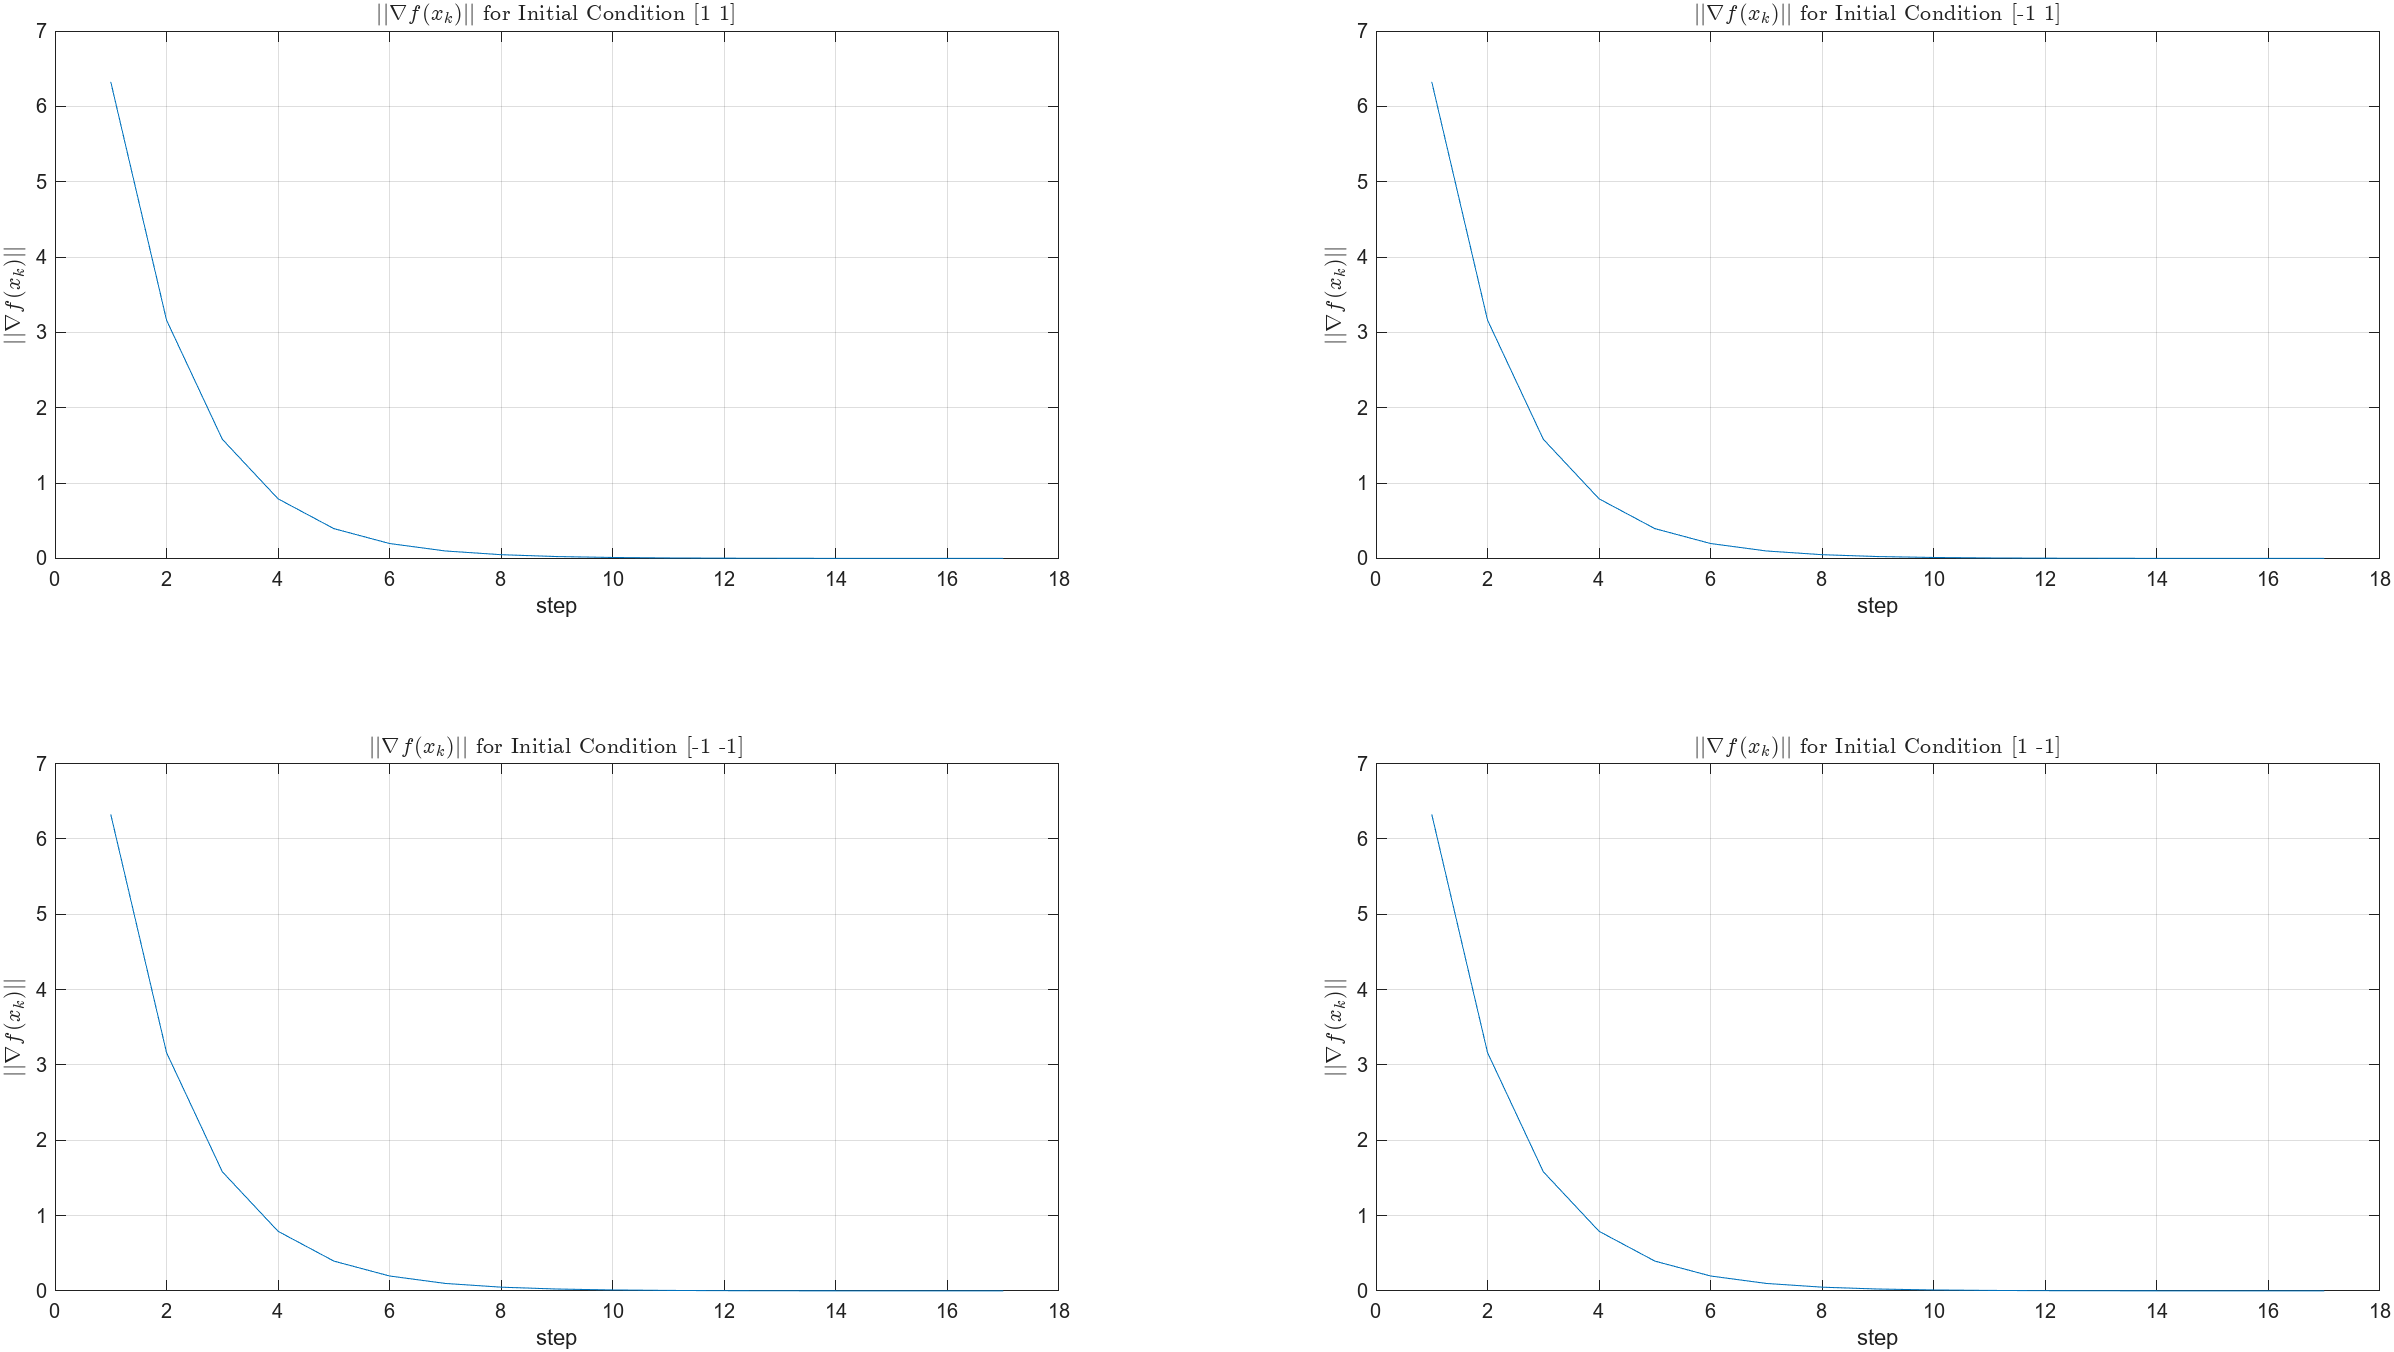
\includegraphics[width = 0.9\textwidth]{Plots/NormGradient.png}
    \caption{Sequence of Normed Gradients for all initial conditions. }
    \label{fig:normedGradient}
\end{figure}
\clearpage
\newpage
\begin{figure}
    \centering
    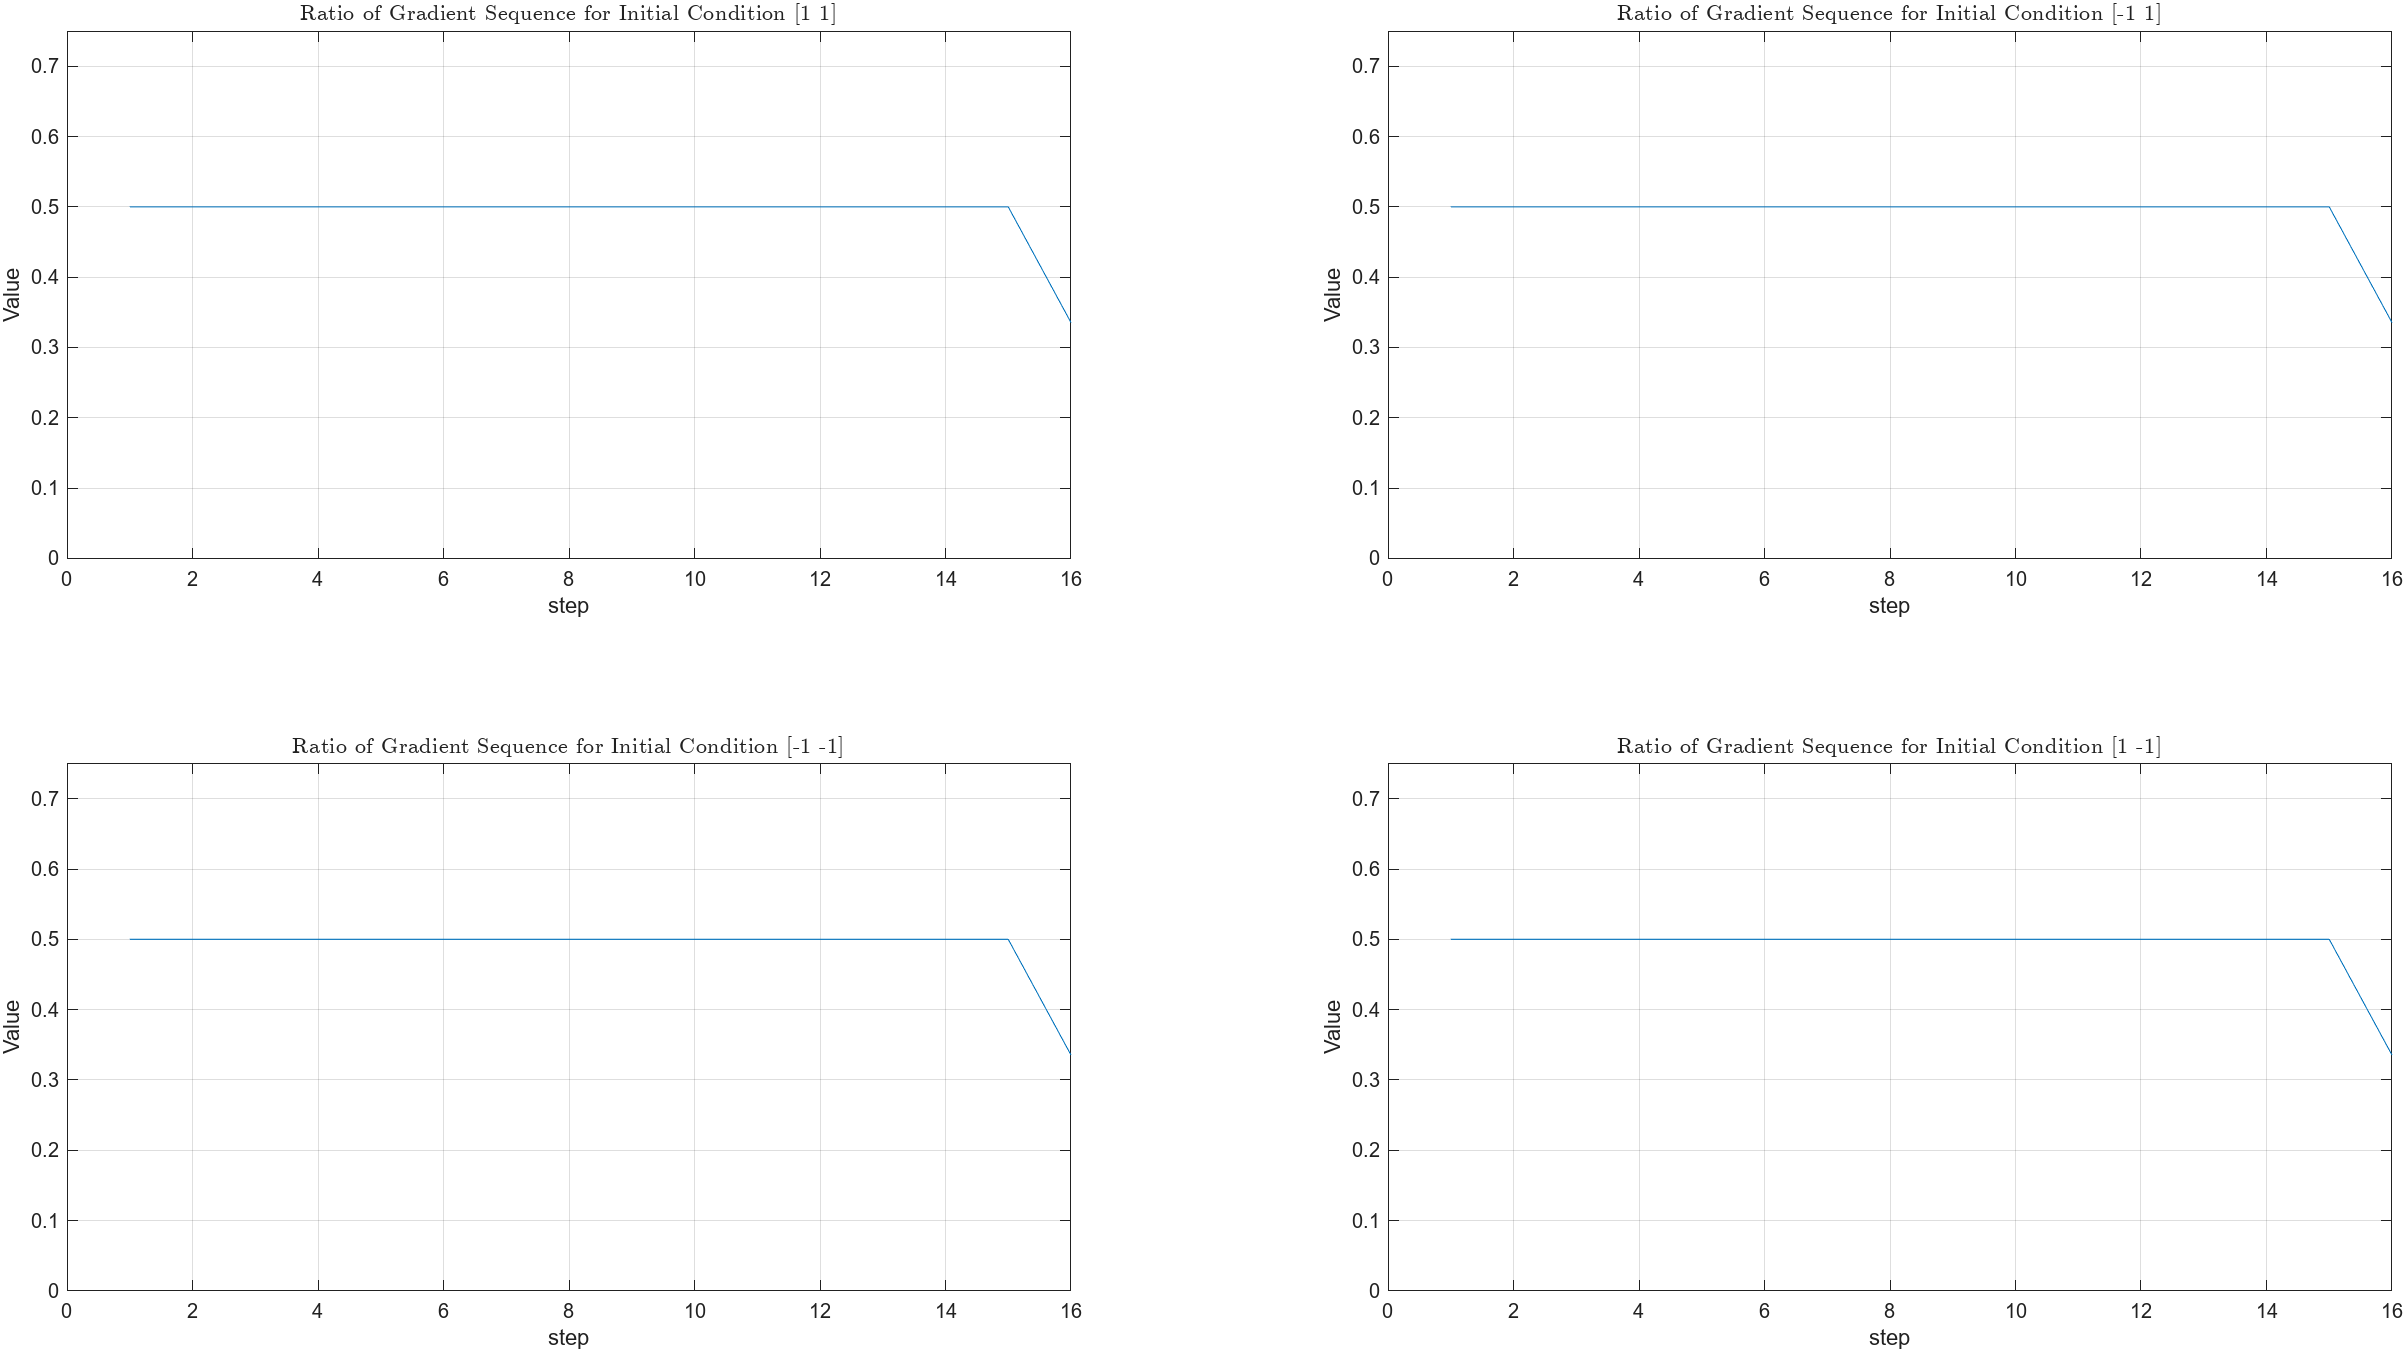
\includegraphics[width = 0.9\textwidth]{Plots/RatioSeq.png}
    \caption{Ratio of Gradient Sequences.}
    \label{fig:RatioSeq}
\end{figure}
\clearpage
\newpage
\subsection{Problem 4, part 6}
Repeat part 5 for $c = 1000$.
\partbreak
\begin{solution}

    I have included the plots below. It seems like we reach our tolerance in finite time \footnote{This is set to 1 x 10$^{-4}$ for all plots.} in Figure \ref{fig:NormGradient1000}. Figure \ref{fig:PlotSeq1000} is somewhat less assuring, however. When zooming in, there is one point that pops up, then it goes back down to a value roughly 0.96. It might be the case that backtracking gives us a stepsize too large, which might get in the say of correctly finding the minima nicely. Figure \ref{fig:Zoomin} is a zoom-in on one of the initial conditions. We can see that there is a ``zig-zag" pattern in the sequence. It is normal for steepest descent algorithms to have this, as discussed in class. 
\end{solution}
\vspace{2cm}
\begin{figure}[!h]
    \centering
    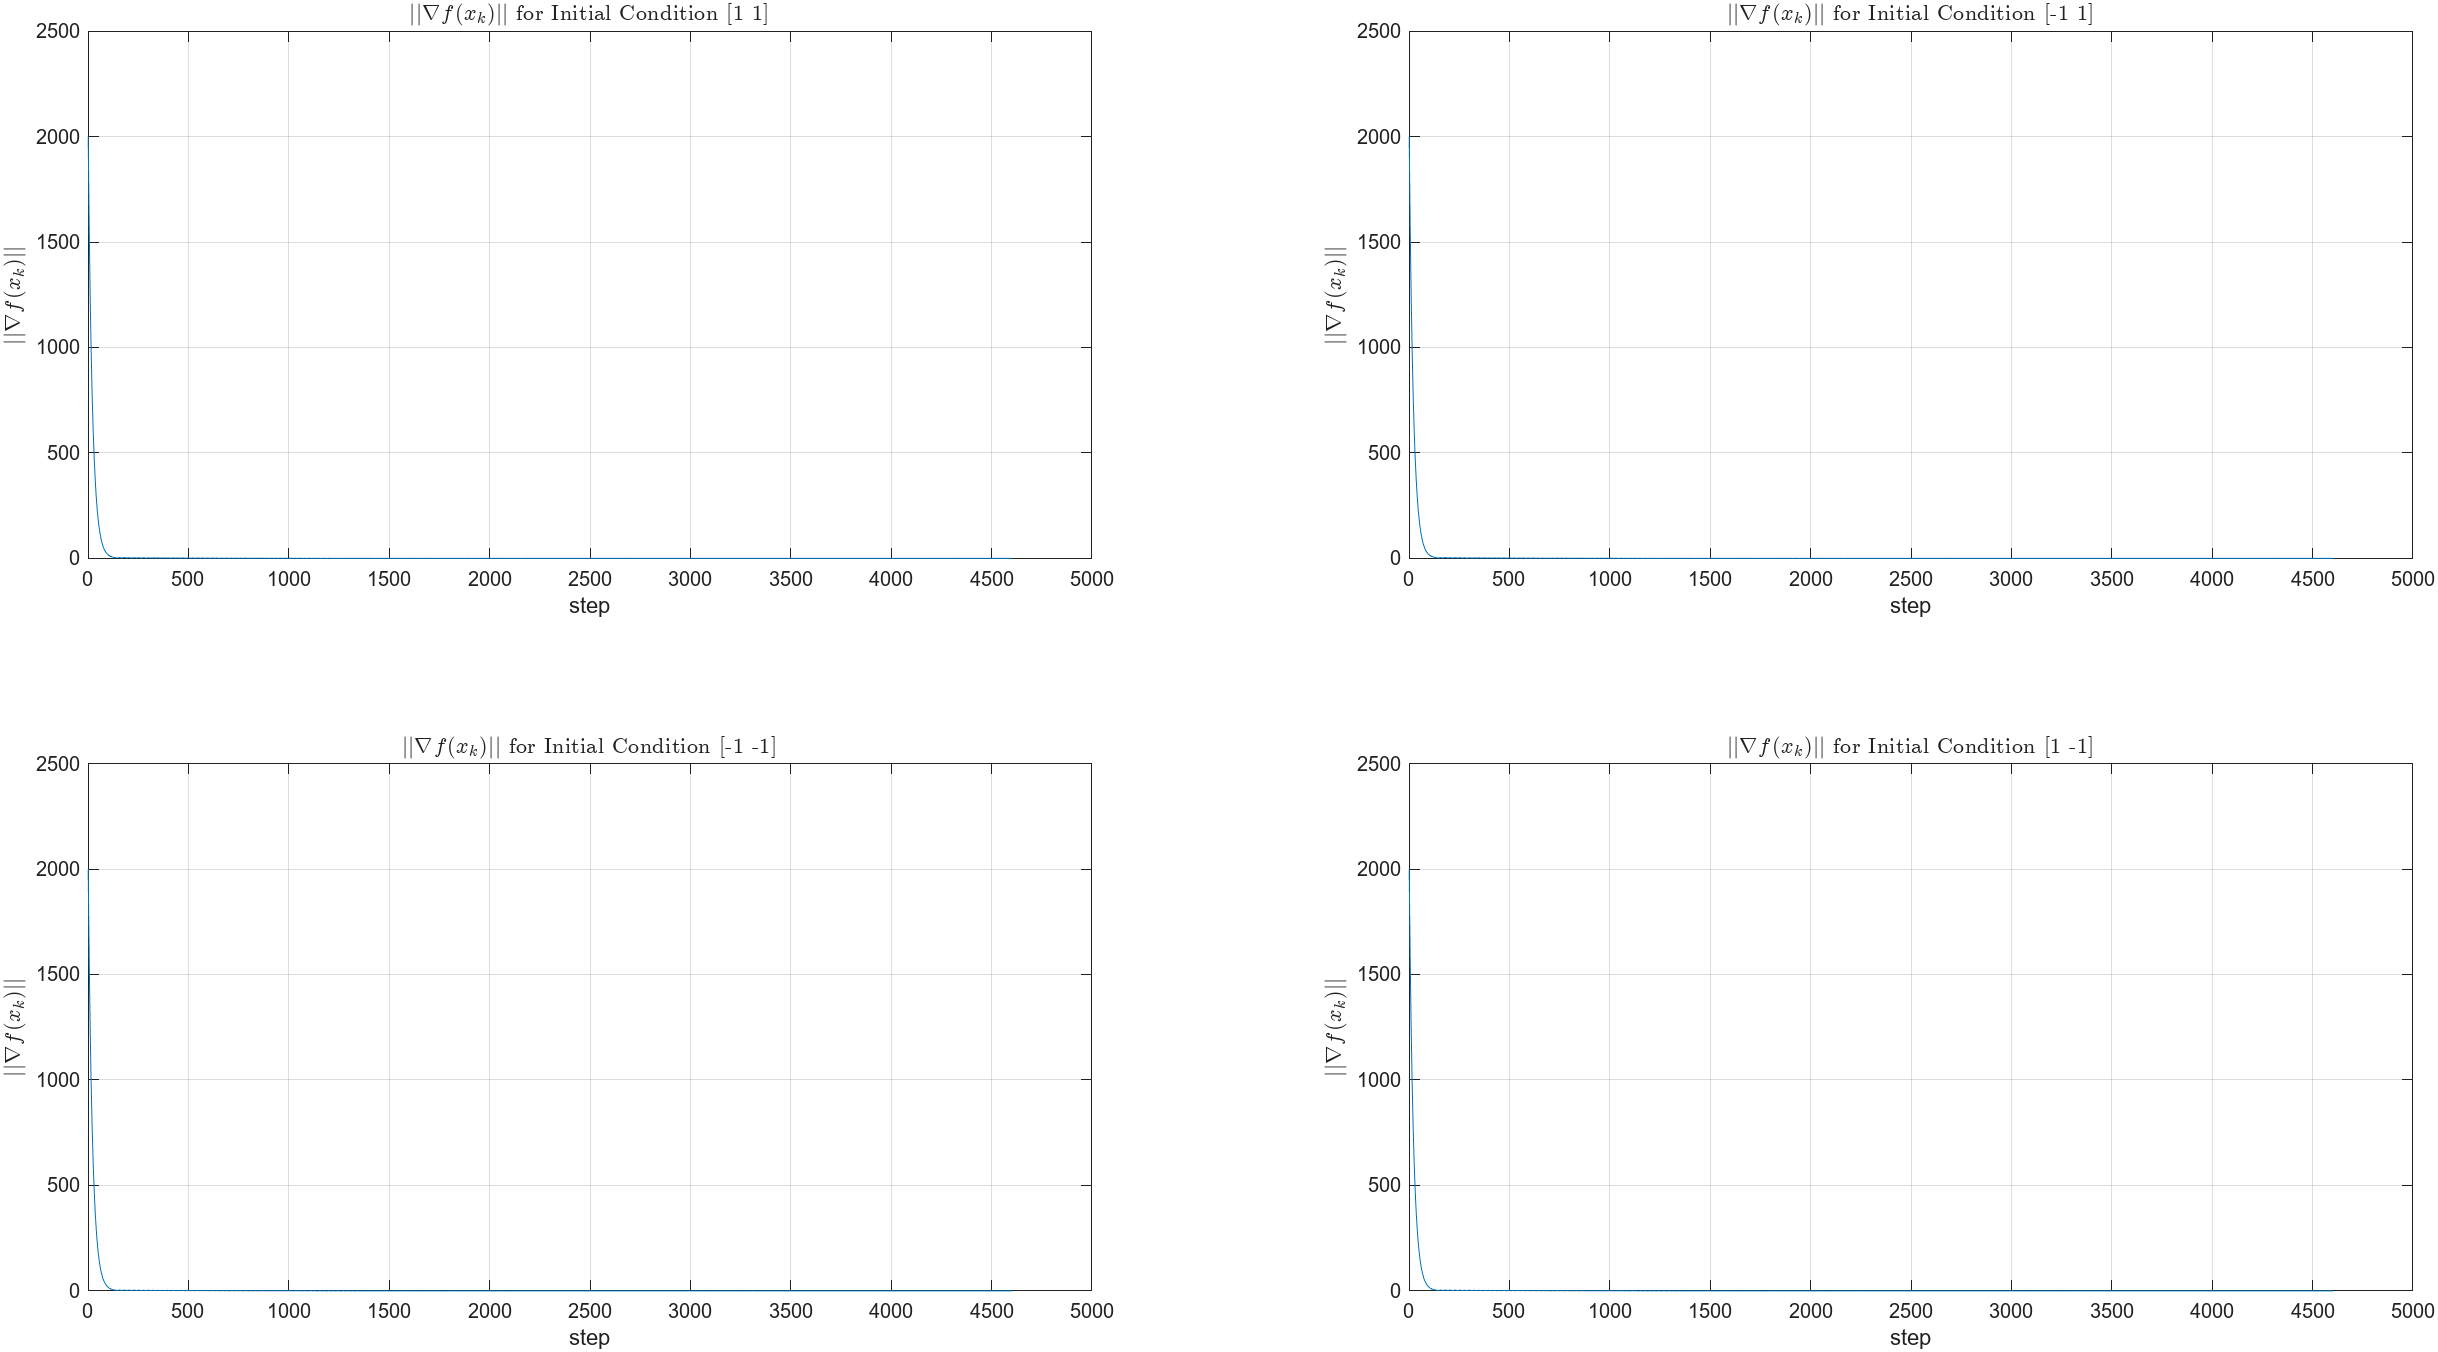
\includegraphics[width = 0.9\textwidth]{Plots/NormGradient1000.png}
    \caption{Sequence of Normed Gradients for all initial conditions with $c = 1000$.}
    \label{fig:NormGradient1000}
\end{figure}

\clearpage
\newpage
\begin{figure}
    \centering
    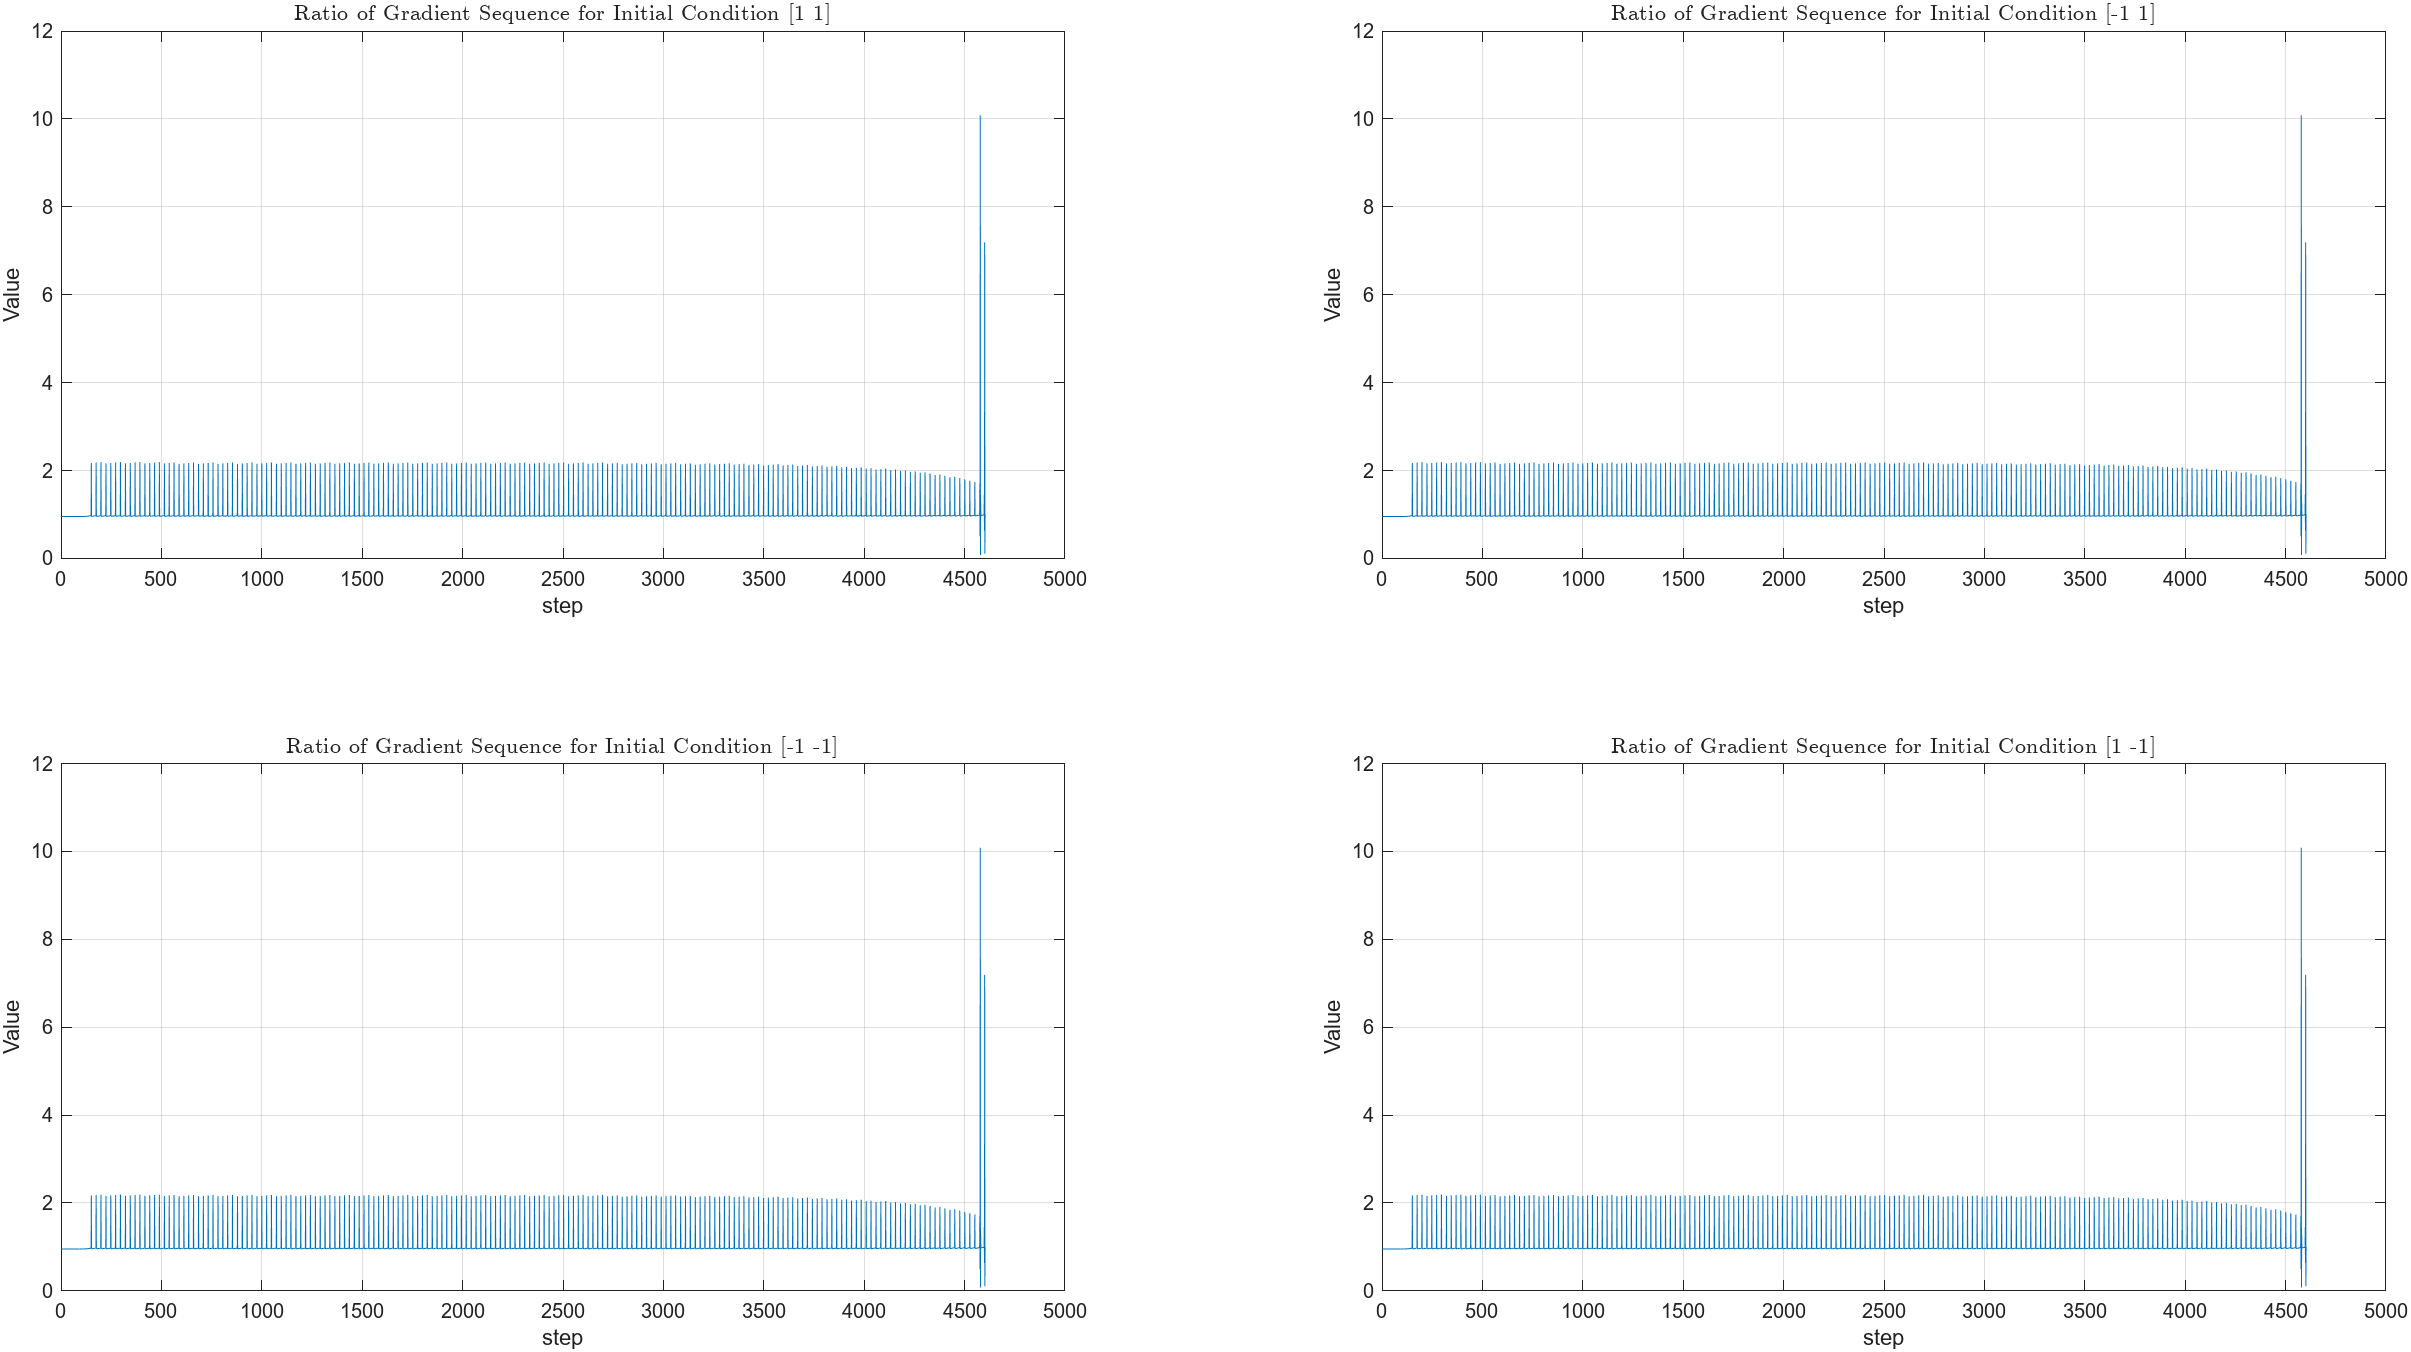
\includegraphics[width = 0.9\textwidth]{Plots/RatioSeq1000.png}
    \caption{Ratio of Gradient Sequences with $c = 1000$.}
    \label{fig:PlotSeq1000}
\end{figure}

\begin{figure}
    \centering
    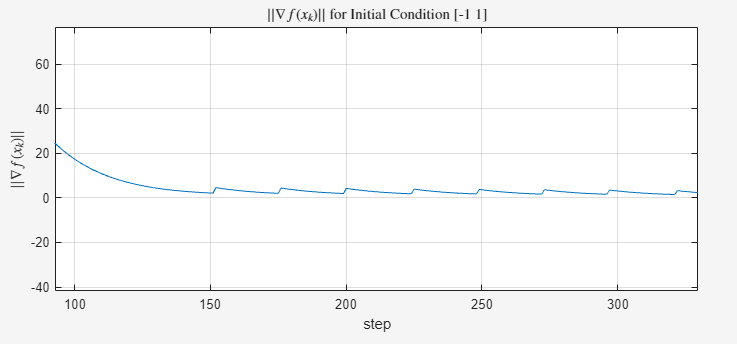
\includegraphics[width = 0.9\textwidth]{Plots/NormGradient1000_zoomin.png}
    \caption{A zoom in on the sequence of normed gradients. We can see the zig-zag pattern that steepest descent is known for.}
    \label{fig:Zoomin}
\end{figure}
\end{document}